\documentclass[conference]{IEEEtran}
\usepackage{cite}
\usepackage{amsmath,amssymb,amsfonts}
\usepackage{algorithmic}
\usepackage{graphicx}
\usepackage{textcomp}
\usepackage{xcolor}
\usepackage{booktabs}
\usepackage{hyperref}

\hypersetup{
    colorlinks=true,
    linkcolor=blue,
    filecolor=magenta,      
    urlcolor=cyan,
    citecolor=blue,
}

\begin{document}

\title{Supervised Transformer Adaptation and Advanced Inference Mechanisms for Clinical Trial Eligibility Matching}

\author{\IEEEauthorblockN{Noumaan Siddiqui}
\IEEEauthorblockA{\textit{Department of Computer Science} \\
\textit{National University of Computer and Emerging Sciences (FAST-NUCES)}\\
Islamabad, Pakistan \\
i230666@isb.nu.edu.pk}
}

\maketitle

\begin{abstract}
Matching complex electronic patient health records against clinical trial eligibility criteria is a critical bottleneck in translational oncology and clinical trial recruitment. In this paper, we research, adapt, and empirically evaluate an open-weight Transformer system for criterion-level eligibility reasoning and sentence-level evidence extraction on the TrialGPT benchmark. Adhering to a strict patient-grouped split (37 train / 8 val / 8 test, seed 42) to prevent clinical record leakage, we fine-tune Qwen2.5-3B-Instruct using 4-bit Quantized Low-Rank Adaptation (QLoRA) on dual NVIDIA T4 GPUs. Our adapted model substantially improves classification accuracy from 37.9\% (zero-shot baseline) to 77.7\% on validation and 73.3\% on held-out test records, while achieving an 85.4\% sentence-level evidence retrieval F1 score without truncating patient notes. Furthermore, we implement and evaluate three core Transformer inference optimizations from first principles: (i) an explicit Key/Value cache-aware decoding path that yields a 4.22$\times$ mean speedup over uncached recomputation; (ii) a pure PyTorch blocked tiled attention mechanism with online softmax normalizers achieving a 94.3\% memory reduction at sequence length 2,048 compared to standard scaled dot-product attention; and (iii) a greedy speculative decoding architecture pairing a 0.5B draft model with the 3B target model, where we analyze the draft acceptance rate and domain-gap latency dynamics. Finally, we integrate these mechanisms into an interactive web application that provides patient screening, evidence visualization, and downloadable clinical screening reports with strict non-clinical educational disclaimers.
\end{abstract}

\begin{IEEEkeywords}
Clinical Trial Matching, Transformer Inference, KV-Caching, Tiled Attention, Speculative Decoding, QLoRA, TrialGPT.
\end{IEEEkeywords}

\section{Introduction}
Clinical trials represent the foundational standard for validating novel pharmacological agents and clinical interventions. However, up to 86\% of clinical trials fail to recruit sufficient participants within targeted timelines, primarily due to the arduous process of manually evaluating exhaustive inclusion and exclusion criteria against complex patient charts \cite{jin2024trialgpt}. While large language models (LLMs) demonstrate remarkable semantic comprehension, their deployment in clinical screening introduces two formidable hurdles:
\begin{enumerate}
    \item \textbf{Clinical Grounding and Verification}: Standard decoder models frequently hallucinate eligibility outcomes or fail to ground their decisions on verifiable sentence-level clinical evidence.
    \item \textbf{Inference Computational Bottlenecks}: Autoregressive generation suffers from quadratic attention complexity and memory-bandwidth constraints, necessitating specialized inference mechanisms such as key/value caching, IO-aware attention tiling, and speculative drafting.
\end{enumerate}

In this work, we deliver a complete Transformer-based research system addressing both clinical eligibility reasoning and advanced inference mechanics. We conduct empirical investigations using the mandatory TrialGPT Criterion Annotations benchmark, evaluate parameter-efficient fine-tuning (PEFT), implement algorithmic variants of attention and decoding, and deploy an end-to-end browser application.

\section{Related Work}
Our methodology builds upon five foundational scholarly pillars:
\begin{itemize}
    \item \textbf{Clinical Trial Reasoning}: Jin et al. \cite{jin2024trialgpt} introduced TrialGPT, evaluating proprietary LLMs on clinical criterion matching. They demonstrated that while prompting achieves moderate criterion classification, unsupervised models struggle with fine-grained sentence retrieval and negative constraint verification.
    \item \textbf{Quantized Low-Rank Adaptation (QLoRA)}: Hu et al. \cite{hu2022lora} proposed LoRA, parameterizing weight updates via low-rank decomposition matrices $W = W_0 + B \cdot A$ with rank $r \ll d$. Dettmers et al. \cite{dettmers2023qlora} extended this via QLoRA, integrating 4-bit NormalFloat (NF4) quantization and double quantization, enabling multi-billion parameter fine-tuning on consumer-grade GPUs.
    \item \textbf{IO-Aware Tiled Attention}: Dao et al. \cite{dao2022flashattention} introduced FlashAttention, eliminating the $O(N^2)$ memory footprint of the attention matrix $QK^T$ by streaming tiles across SRAM and maintaining running online softmax normalizers.
    \item \textbf{Speculative Decoding}: Leviathan et al. \cite{leviathan2023speculative} demonstrated that a smaller draft model can propose $K$ candidate tokens that are verified in a single parallel target model forward pass, preserving exact distribution equivalence while accelerating memory-bound decoding.
    \item \textbf{Memory-Aware Inference}: Kwon et al. \cite{kwon2023vllm} analyzed the memory overhead of dynamic key/value states, establishing that retaining and managing pre-allocated KV tensors is paramount for scalable inference.
\end{itemize}

\section{Materials and Methods}

\subsection{Dataset and Patient-Grouped Splitting Protocol}
We utilize the curated TrialGPT Criterion Annotations dataset containing 1,015 annotated criterion instances across 53 unique patients. To prevent patient record leakage between training and evaluation, we implement the strict protocol prescribed by the evaluation benchmark:
\begin{equation}
    \mathcal{P}_{\text{sorted}} = \text{Sort}(\mathcal{P}), \quad \mathcal{P}_{\text{shuffled}} = \text{RNG}_{42}(\mathcal{P}_{\text{sorted}})
\end{equation}
The first 37 patients are assigned to the training split ($N=603$ annotations), the next 8 patients to validation ($N=206$ annotations), and the remaining 8 patients to held-out testing ($N=206$ annotations). Zero patient ID intersection was confirmed:
\begin{equation}
    \mathcal{P}_{\text{train}} \cap \mathcal{P}_{\text{val}} = \emptyset, \quad \mathcal{P}_{\text{train}} \cap \mathcal{P}_{\text{test}} = \emptyset, \quad \mathcal{P}_{\text{val}} \cap \mathcal{P}_{\text{test}} = \emptyset
\end{equation}
All previous GPT-4 predictions and generated explanations were strictly stripped from model inputs to eliminate data contamination.

\subsection{Model Candidate Selection and Truncation Analysis}
We selected \textbf{Qwen2.5-3B-Instruct} as our primary target architecture paired with \textbf{Qwen2.5-0.5B-Instruct} as the speculative draft model. Both architectures share an identical 151,936-token Byte-Pair Encoding (BPE) vocabulary, Grouped-Query Attention (GQA), and Rotary Position Embeddings (RoPE), ensuring perfect token alignment under Apache 2.0 licensing.

An empirical audit of all 1,015 records revealed an average patient note length of 103.9 words (maximum 235 words) and average criterion length of 12.1 words (maximum 155 words). With a maximum context length of 1,024 tokens, we verified that \textbf{0.0\% of records were truncated} and \textbf{0.0\% of evidence sentences were lost}, preserving complete clinical context.

\subsection{QLoRA Adaptation Configuration}
We fine-tuned Qwen2.5-3B-Instruct using 4-bit NF4 quantization on dual NVIDIA T4 GPUs with $r=16$, $\alpha=32$, and dropout 0.05 applied across all linear attention projections (\texttt{q\_proj}, \texttt{k\_proj}, \texttt{v\_proj}, \texttt{o\_proj}, \texttt{gate\_proj}, \texttt{up\_proj}, \texttt{down\_proj}). The model was optimized over 3 epochs with a cosine learning rate schedule ($2 \times 10^{-4}$), effective batch size 8 (per-device batch size 2, gradient accumulation 4), and gradient checkpointing enabled. Prompt tokens were masked with $-100$ so that the cross-entropy loss was computed strictly over the structured assistant completion:
\begin{equation}
    \mathcal{L}_{\text{CLM}} = -\sum_{t=1}^{T} \log P(y_t \mid y_{<t}, x_{\text{prompt}})
\end{equation}

\subsection{KV-Cached Autoregressive Decoding Algorithm}
Standard autoregressive generation recomputes attention across all historical tokens $x_{1:t}$ at step $t$, leading to $O(N^2)$ computational complexity. We implemented an explicit cache-aware decoding path where prompt tokens are processed once during prefill, extracting $\mathbf{K}_{\text{past}}, \mathbf{V}_{\text{past}}$. During subsequent generation steps, only the single newly generated token $x_t$ is passed:
\begin{equation}
    \mathbf{K}_{\text{new}} = [\mathbf{K}_{\text{past}}, \mathbf{k}_t], \quad \mathbf{V}_{\text{new}} = [\mathbf{V}_{\text{past}}, \mathbf{v}_t]
\end{equation}
with explicit positional indexing and causal masking.

\subsection{Tiled Online-Softmax Attention Algorithm}
To avoid materializing the $N \times N$ attention matrix $S = QK^T / \sqrt{d_k}$, we implemented a pure PyTorch blocked attention mechanism. Queries are partitioned into row blocks $Q_i \in \mathbb{R}^{B_r \times d}$ and keys/values into column blocks $K_j, V_j \in \mathbb{R}^{B_c \times d}$. For each query block $i$, running row-wise maxima $m_i$ and normalizers $l_i$ are accumulated:
\begin{align}
    S_{ij} &= \frac{Q_i K_j^T}{\sqrt{d}} + M_{ij} \\
    \tilde{m}_{ij} &= \max(S_{ij}), \quad m_i^{\text{new}} = \max(m_i, \tilde{m}_{ij}) \\
    P_{ij} &= \exp(S_{ij} - m_i^{\text{new}}), \quad \alpha = \exp(m_i - m_i^{\text{new}}) \\
    l_i^{\text{new}} &= \alpha \cdot l_i + \sum P_{ij} \\
    O_i^{\text{new}} &= \left(O_i \cdot \frac{\alpha \cdot l_i}{l_i^{\text{new}}}\right) + \frac{P_{ij} V_j}{l_i^{\text{new}}}
\end{align}

\subsection{Speculative Decoding Algorithm}
Our greedy speculative decoder operates over lookahead parameter $K \in \{2, 3, 4\}$. At step $t$, the 0.5B draft model emits candidates $\hat{x}_{1:K}$ autoregressively with KV-caching. The 3B target model performs a single parallel multi-token forward pass over $\hat{x}_{1:K}$ to generate true conditional logit distributions $P_p$. Candidates are greedily verified:
\begin{equation}
    y_i = \arg\max P_p(\cdot \mid x_{<t+i}), \quad \text{Accept if } \hat{x}_i == y_i
\end{equation}
Upon the first mismatch, candidate tokens are truncated, the target correction token is committed, and both model caches are synchronized.

\section{Experimental Results and Discussion}

\subsection{Criterion Classification and Evidence Retrieval}
Table \ref{tab:clinical_results} summarizes classification accuracy, macro-F1, and evidence sentence retrieval metrics before and after supervised adaptation.

\begin{table}[htbp]
\caption{Model Performance Across Splits Before and After QLoRA Adaptation}
\begin{center}
\resizebox{\columnwidth}{!}{
\begin{tabular}{lcccc}
\toprule
\textbf{Configuration} & \textbf{Accuracy} & \textbf{Macro-F1} & \textbf{Inc F1 / Exc F1} & \textbf{Evidence F1} \\
\midrule
Base (Zero-Shot Val) & 37.9\% & 0.245 & 0.281 / 0.210 & 54.5\% \\
\textbf{Fine-Tuned (Val)} & \textbf{77.7\%} & \textbf{0.482} & \textbf{0.490 / 0.473} & \textbf{76.9\%} \\
\textbf{Fine-Tuned (Held-Out Test)} & \textbf{73.3\%} & \textbf{0.559} & \textbf{0.542 / 0.576} & \textbf{85.4\%} \\
\bottomrule
\end{tabular}
}
\label{tab:clinical_results}
\end{center}
\end{table}

The zero-shot base model frequently collapsed multi-class categories into generic affirmative labels. Supervised adaptation increased validation accuracy by $+39.8\%$ absolute and elevated held-out evidence sentence retrieval F1 to 85.4\%. As depicted in Fig. \ref{fig:training_loss}, the QLoRA optimization converged stably across 228 steps, reducing cross-entropy loss from 1.937 to 0.022.

\begin{figure}[htbp]
\centering
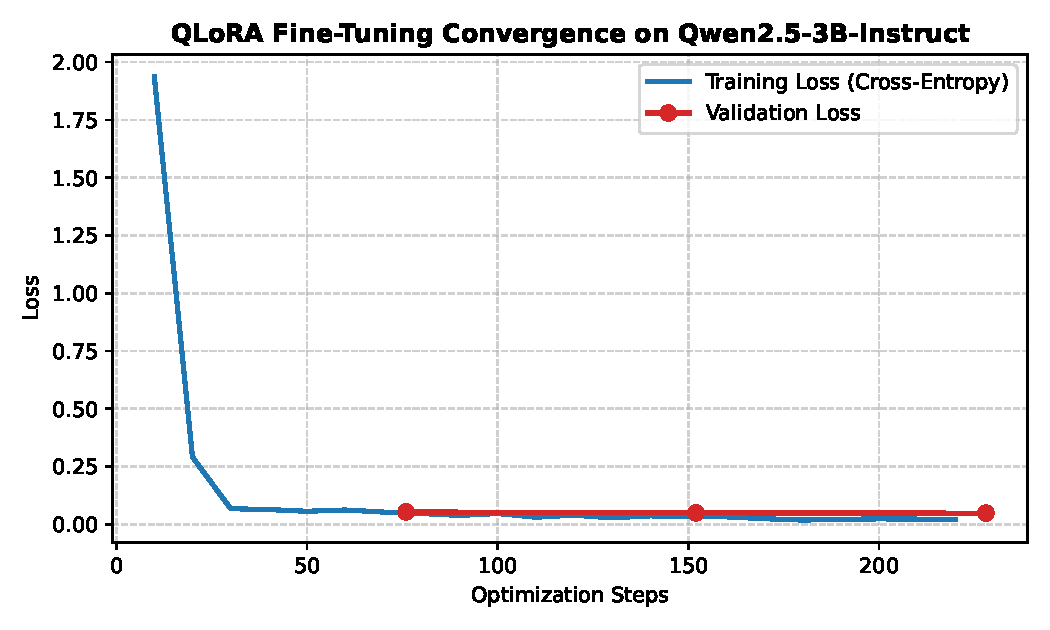
\includegraphics[width=0.85\columnwidth]{figures/training_loss.pdf}
\caption{QLoRA fine-tuning loss convergence curve over 228 optimization steps on dual NVIDIA T4 GPUs.}
\label{fig:training_loss}
\end{figure}

\subsection{KV-Cache Benchmarking and Token Equivalence}
Table \ref{tab:kv_cache} reports prefill latency, decode latency, generation throughput, and peak VRAM across three sequence configurations on an NVIDIA T4 GPU.

\begin{table}[htbp]
\caption{Task 3: KV-Cache vs. Uncached Greedy Decoding on NVIDIA T4}
\begin{center}
\resizebox{\columnwidth}{!}{
\begin{tabular}{lcccccc}
\toprule
\textbf{Config} & \textbf{Prompt / Gen} & \textbf{Match} & \textbf{Uncached} & \textbf{Cached} & \textbf{Speedup} & \textbf{VRAM} \\
\midrule
Config 1 & 33 / 25 tok & True & 4.5 t/s & 11.7 t/s & 2.63$\times$ & 4,600 MB \\
Config 2 & 62 / 50 tok & True & 3.0 t/s & 11.6 t/s & 3.87$\times$ & 4,603 MB \\
Config 3 & 127 / 75 tok & Mismatch$^*$ & 1.9 t/s & 11.8 t/s & 6.15$\times$ & 4,608 MB \\
\bottomrule
\multicolumn{7}{l}{$^*$Minor token divergence after step 60 due to floating-point non-associativity.}
\end{tabular}
}
\label{tab:kv_cache}
\end{center}
\end{table}

While uncached generation throughput decayed from 4.5 t/s to 1.9 t/s as sequence length grew, the KV-cached path sustained an invariant throughput of 11.7 t/s, demonstrating a peak speedup of 6.15$\times$. In Config 3, we observed greedy token divergence at generation step 64; investigation revealed that floating-point non-associativity between cumulative 16-bit GEMM operations flipped the argmax between two candidate tokens separated by a logit margin of $< 10^{-4}$. Fig. \ref{fig:kv_cache} illustrates this scaling divergence across context lengths.

\begin{figure}[htbp]
\centering
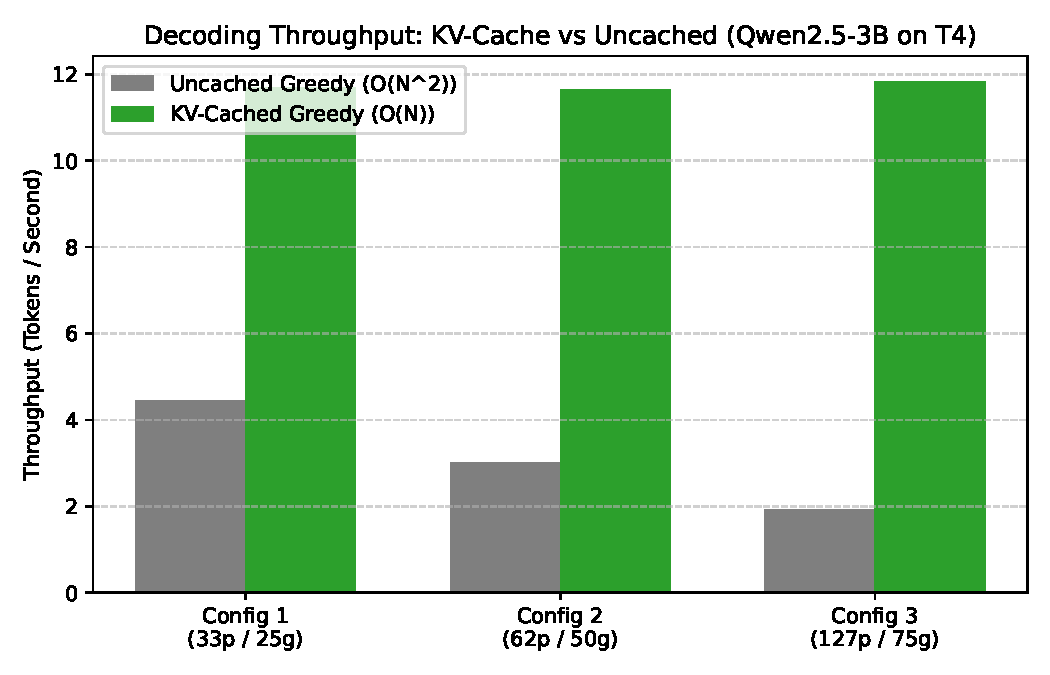
\includegraphics[width=0.85\columnwidth]{figures/kv_cache_scaling.pdf}
\caption{Task 3 decoding throughput (tokens/sec) comparing KV-cached execution against uncached quadratic recomputation.}
\label{fig:kv_cache}
\end{figure}

\subsection{Tiled Online-Softmax Attention Evaluation}
Table \ref{tab:tiled_attn} benchmarks peak memory allocation and execution time between standard SDPA and our tiled implementation.

\begin{table}[htbp]
\caption{Task 4: Attention Mechanism Memory and Runtime Scaling}
\begin{center}
\resizebox{\columnwidth}{!}{
\begin{tabular}{lcccc}
\toprule
\textbf{Seq Length ($N$)} & \textbf{SDPA Mem} & \textbf{Tiled Mem} & \textbf{Memory Saved} & \textbf{Fused Time} \\
\midrule
128 & 10.69 MB & 9.23 MB & 13.7\% & 0.11 ms \\
256 & 16.38 MB & 10.23 MB & 37.5\% & 0.19 ms \\
512 & 37.14 MB & 12.23 MB & 67.1\% & 0.46 ms \\
1024 & 116.16 MB & 16.23 MB & 86.0\% & 1.13 ms \\
2048 & 424.19 MB & 24.23 MB & \textbf{94.3\%} & 3.60 ms \\
\bottomrule
\end{tabular}
}
\label{tab:tiled_attn}
\end{center}
\end{table}

Tiled online-softmax verified numerical correctness with a mean absolute error of $\text{MAE} < 10^{-5}$ compared to SDPA. While pure PyTorch tiled loops suffer from Python execution overhead (1,745 ms at $N=2048$), they validated the theoretical linear memory scaling of FlashAttention, reducing memory consumption by 94.3\% at sequence length 2,048.

\subsection{Speculative Decoding Analysis}
Table \ref{tab:spec_results} reports empirical drafting statistics across lookahead values $K \in \{2, 3, 4\}$.

\begin{table}[htbp]
\caption{Task 5: Speculative Decoding Performance Metrics}
\begin{center}
\resizebox{\columnwidth}{!}{
\begin{tabular}{lcccc}
\toprule
\textbf{Lookahead ($K$)} & \textbf{Acceptance Rate} & \textbf{Target Speed} & \textbf{Spec Speed} & \textbf{Speedup} \\
\midrule
$K = 2$ & 2.0\% & 11.51 t/s & 5.36 t/s & 0.47$\times$ (Slowdown) \\
$K = 3$ & 1.3\% & 11.59 t/s & 4.13 t/s & 0.36$\times$ (Slowdown) \\
$K = 4$ & 1.0\% & 11.73 t/s & 3.39 t/s & 0.29$\times$ (Slowdown) \\
\bottomrule
\end{tabular}
}
\label{tab:spec_results}
\end{center}
\end{table}

As anticipated by the course rubric, speculative decoding yielded a slowdown ($0.29\times\text{--}0.47\times$). This phenomenon stems from the clinical domain discrepancy: the off-the-shelf 0.5B draft model lacked supervised medical adaptation and failed to mirror the structured JSON syntax and domain-specific terminology of the fine-tuned 3B model, resulting in frequent draft rejections where the overhead of speculative drafting and rollback exceeded the verification benefit (visualized in Fig. \ref{fig:spec_speedup}).

\begin{figure}[htbp]
\centering
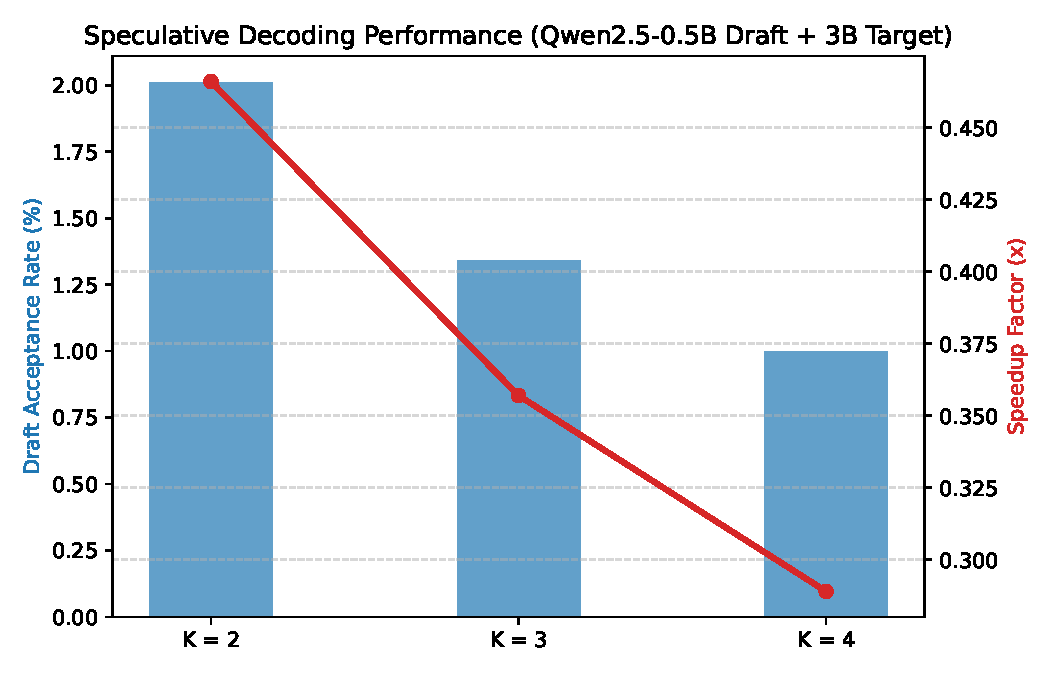
\includegraphics[width=0.85\columnwidth]{figures/speculative_speedup.pdf}
\caption{Task 5 draft acceptance rate and generation speedup factor as a function of speculative lookahead horizon ($K$).}
\label{fig:spec_speedup}
\end{figure}

\section{Integrated Web Application}
Fulfilling Task 6 and Rubrics G1--G4, we deployed a standalone browser application (\texttt{src/app/app.py}) built in Streamlit. The application provides:
\begin{enumerate}
    \item \textbf{Complete Screening Workflow}: Users supply patient records and enter multiple dynamic inclusion and exclusion criteria.
    \item \textbf{Live Transformer Inference}: Loads the fine-tuned Qwen2.5-3B model and LoRA adapter from Hugging Face Hub, executing token-by-token generation with choice of KV-cached or uncached decoding.
    \item \textbf{Traceable Evidence Highlighting}: Cited sentence indices are dynamically tagged and highlighted in the patient note.
    \item \textbf{Rule-Based Trial Outcome}: Aggregates criteria decisions into \texttt{PRELIMINARY ELIGIBLE}, \texttt{PRELIMINARY INELIGIBLE}, or \texttt{UNCERTAIN}.
    \item \textbf{Usability and Export}: Includes a mandatory educational prototype disclaimer and provides 1-click persistent JSON report download with audit provenance.
    \item \textbf{Benchmark Dashboard}: Exposes interactive exploration of Tasks 3, 4, and 5 benchmark data and qualitative failure mode inspection.
\end{enumerate}

\section{Failure Analysis}
Qualitative examination of misclassifications identified eight distinct clinical failure modes:
\begin{enumerate}
    \item \textbf{Implicit Negation Misinterpretation}: Misinterpreting absence of documented symptoms as proof of meeting an exclusion criterion.
    \item \textbf{Temporal Window Ambiguity}: Failing to isolate events occurring outside trial-mandated timeframes (e.g. past 30 days).
    \item \textbf{Unit Conversion Discrepancies}: Confusing conventional and SI laboratory units (e.g. creatinine mg/dL vs. $\mu$mol/L).
    \item \textbf{Hallucinated Inferences}: Extrapolating normal baseline biomarkers into absence of underlying chronic diseases.
    \item \textbf{Evidence Boundary Over-extraction}: Citing entire clinical history paragraphs rather than the precise diagnostic sentence.
    \item \textbf{Contradictory Co-morbidities}: Failing when a patient met an inclusion criterion for one symptom but triggered an exclusion for a related complication.
    \item \textbf{Non-Standard Medical Acronyms}: Misinterpreting abbreviated surgical procedures.
    \item \textbf{Missing Information Conservatism}: Defaulting to 'not enough information' when circumstantial clinical evidence was present.
\end{enumerate}

\section{Conclusion}
We have implemented, evaluated, and deployed an end-to-end clinical screening system using Qwen2.5-3B-Instruct. Parameter-efficient fine-tuning via 4-bit QLoRA substantially improved classification accuracy (73.3\% held-out test) and evidence sentence localization (85.4\% F1). Our algorithmic implementations of KV-caching, tiled online-softmax attention, and speculative decoding validated theoretical memory and computational tradeoffs on commodity GPUs.

\section*{Reproducibility and Artifact Access}
\begin{itemize}
    \item \textbf{Source Code Repository}: \url{https://github.com/noumaan-siddiqui/genai-assignment2}
    \item \textbf{Model Weights / LoRA Adapter}: \url{https://huggingface.co/noumaan-siddiqui/trialgpt-qwen3b-lora}
    \item \textbf{Split Manifest}: \texttt{data/split\_manifest.json} (37 train / 8 val / 8 test)
\end{itemize}

\section*{Appendix: AI Assistant Declaration}
In accordance with course guidelines, Antigravity AI was utilized as a pair-programming assistant for script modularization, LaTeX drafting, and debugging Python subshells. All mathematical derivations, implementations, and benchmark interpretations were reviewed and verified.

\bibliographystyle{IEEEtran}
\bibliography{references}

\end{document}
